\documentclass[12pt,french]{report}
\input preambule_17-18
\input{perso_cecile_2017}
\input{commandes_17-18}

\newgeometry{includeheadfoot,headsep=0.2cm,top=0.5cm,bottom=0.8cm,right=1.5cm,left=1.5cm}
\pagestyle{fancy}
\fancyhf{}

\ReglePied

\fancypagestyle{garde}{
\entete{\small\textbf{Nom,  Prénom :} \makebox[5cm]{\dotfill}} {}{\small \textbf{Classe} }

\pieddepage{2018-2019 }{}{\thepage / \pageref{LastPage}}}

\pieddepage{2018-2019 - Classe}{DS }{\thepage / \pageref{LastPage}}









\begin{document}
\thispagestyle{garde}

\medskip

%cadre titre
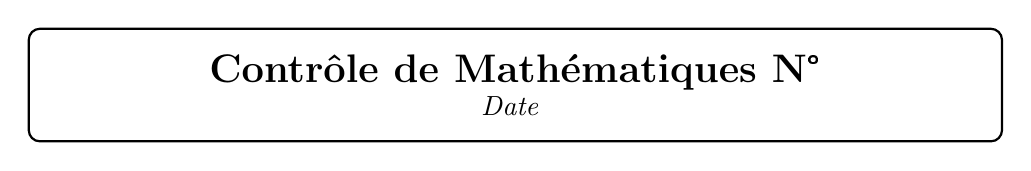
\begin{tikzpicture}
\node[rectangle,draw=black,rounded corners,thick,fill=white]{%
\begin{minipage}{\linewidth}
\begin{center}
\vspace*{6pt}
\textbf{\Large \bsc{Contrôle de Mathématiques} N°}\par
\textit{Date}
\vspace*{6pt}
\end{center}
\end{minipage}
};\end{tikzpicture}





% consignes

\begin{center}
\begin{minipage}{0.8\linewidth}
\begin{center}
\itshape
%\textbf{Les calculatrices ne sont pas autorisées}.\par
La qualité de la rédaction, la clarté et la précision des raisonnements seront prises en compte dans l'appréciation de la copie.
Le barème est indicatif.
\end{center}
\end{minipage}
\end{center}




%$$$$$$$$ le contrôle !$$$$$$$$$$$$$$$$$$$


%\SetupExSheets[question]{print=false}
%\SetupExSheets[solution]{print=true}

%\printsolutions[byID={• }]

\end{document}
